\section{\texorpdfstring{$k$}{k}-Pebble Transducers}\label{sec:kPebbleTransducers}

We use the notion of \pt{k} as defined in \cite{MSV2000}. For the sake of completeness, we include the definition here.

\begin{definition}
    A \emph{\pt{k}} is a tuple $T := (\alphabet, \alphabet', \automatonStateSet, \automatonInitialState, \automatonTransitionSet)$, where $\alphabet, \alphabet'$ are ranked input and output alphabets respectively, $\automatonStateSet$ is a finite set of \emph{states}, $\automatonInitialState \in \automatonStateSet$ is the \emph{initial state}, and $\automatonTransitionSet$ is a finite set of transitions, each of which has one of the following forms:
    \begin{itemize}
        \item $(a, \vect{b}, q) \to (q', stay)$,
        \item $(a, \vect{b}, q) \to (q', downLeft)$,
        \item $(a, \vect{b}, q) \to (q', downRight)$,
        \item $(a, \vect{b}, q) \to (q'
        , upLeft)$,
        \item $(a, \vect{b}, q) \to (q', upRight)$,
        \item $(a, \vect{b}, q) \to (q', addPebble)$,
        \item $(a, \vect{b}, q) \to (q', removePebble)$,
        \item $(a, \vect{b}, q) \to (a', output0)$,
        \item $(a, \vect{b}, q) \to (a'(q_1, q_2), output2)$,
    \end{itemize}
    where $a \in \alphabet, a' \in \alphabet', \vect{b} \in \bigcup_{i=1}^{k}\set{0,1}^{i-1}$, and $q, q', q_1, q_2 \in Q$.
\end{definition}
\red{Need to define concepts like run, transduction, etc.}

Let $\Gamma$ be a finite alphabet. Let $\rev : \Gamma^* \to \Gamma^*$ be the function defined as follows: For each $w := a_1a_2\dots a_n \in \Gamma^*$ with $a_i \in \Gamma,~\forall i \in [n]$, we let $\rev(w) := a_na_{n-1}\dots a_2a_1$. Let $\Sigma := \Gamma \uplus \set{\#}$ be a finite ranked alphabet with the ranking function $\rank : \Sigma \to \N_0$ given by
\[ \twopartfunc{\rank(a)}{2}{a \in \Gamma}{0}{a = \#} \]
We define the tree-representation-of-string function $\phi : \Gamma^* \to \trees{\alphabet}$ given by defining for $w := a_1a_2\dots a_n \in \Gamma^*$ with $a_i \in \Gamma$, $\phi(w)$ as

\[
\phi(w) := 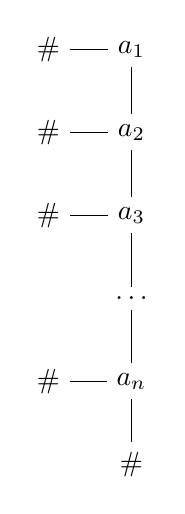
\begin{tikzpicture}
    [level distance=3em]
    \node {$a_1$}
    child[grow=west] { node{$\#$} }
    child[grow=south] {
        node {$a_2$}
        child[grow=west] { node{$\#$} }
        child[grow=south] {
            node{$a_3$}
            child[grow=west] { node{$\#$} }
            child[grow=south] {
                node{$\dots$}
                child[grow=south] {
                    node{$a_n$}
                    child[grow=west] { node{$\#$} }
                    child[grow=south] { node{$\#$} }
                }
            }
        }
    };
\end{tikzpicture}
\]

Note that $\phi$ as defined above is an injective function. We define a function $\widetilde{\rev} : \phi[\Gamma^*] \to \phi[\Gamma^*]$ by setting $\widetilde{\rev} := \phi \circ \rev \circ \phi\inv$. By abuse of notation, we shall write $\widetilde{\rev}$ as just \rev\ when there is no need to distinguish between the two.

\begin{theorem}\cite{MSV2000}
    There exists a \pt{2} $T$ such that $\sem{T}(t) := \rev(t)$ for all $t \in \phi[\Gamma^*]$.
\end{theorem}

\begin{proof}
    Consider the \pt{2} $T$ given by $T := (\alphabet, \alphabet, Q, q_0, \Delta)$ where we have $Q := \set{q_0, q_{up}, q_{down}, q_{out}, q_{lleaf}, q_{rleaf}}$. Since there are only 2 pebbles, the bit-vector $\vec{b}$ has atmost one dimension, which is the presence or absence of the first pebble. Hence we shall denote it as $\top$ or $\bot$ respectively whenever applicable. The transition rules in $\Delta$ are as follows:
    \begin{itemize}
        \item $(a, \emptyset, q_0) \to (q_{down}, addPebble),~ \forall a \in \Gamma,$
        \item $(\#, \emptyset, q_0) \to (\#, output0),$
        \item $(a, \top, q_{down}) \to (q_{down}, downRight),~ \forall a \in \Gamma,$
        \item $(a, \bot, q_{down}) \to (q_{down}, downRight),~ \forall a \in \Gamma,$
        \item $(\#, \bot, q_{down}) \to (q_{out}, upLeft),$
        \item $(a, \bot, q_{out}) \to (a(q_{lleaf}, q_{up}), output2),~ \forall a \in \Gamma,$
        \item $(a, \bot, q_{up}) \to (q_{out}, upLeft),~ \forall a \in \Gamma,$
        \item $(a, \bot, q_{lleaf}) \to (q_{out}, downLeft),~ \forall a \in \Gamma,$
        \item $(\#, \bot, q_{out}) \to (\#, output0),$
        \item $(a, \top, q_{up}) \to (a(q_{lleaf}, q_{rleaf}), output2),~ \forall a \in \Gamma,$
        \item $(a, \top, q_{rleaf}) \to (q_{out}, downRight),~ \forall a \in \Gamma,$
    \end{itemize}
    We can observe that the above \pt{2} $T$ does reverse strings, i.e., $\sem{T}(t) = \rev(t)$ for all $t \in \phi[\Gamma^*]$.
\end{proof}

\begin{theorem}\label{thm:bimorphismCannotReverse}
    There does not exist a triple $(L, \psi_1, \psi_2)$ where $L$ is a regular tree language over a finite ranked alphabet $\Lambda$ and $\psi_1, \psi_2 : \trees{\Lambda} \to \trees{\seedAlphabet}$ are tree homomorphisms and a subset $X \subseteq \trees{\Lambda}$ such that $\set{(\psi_1(t), \psi_2(t)) \mid t \in X} = \rev$.
\end{theorem}

\begin{proof}
Let us assume to the contrary that there exists a triple $(L, \psi_1, \psi_2)$ as specified above such that for a subset $X \subseteq \trees{\Lambda}$, we have $\set{(\psi_1(t), \psi_2(t)) \mid t \in X} = \rev$. Then we see that when $\psi_1, \psi_2$ as homomorphisms are restricted to the set $\Lambda$, $\psi_1(x), \psi_2(x)$ would necessarily have to be trees of height 1, for all $x \in \Lambda$. In other words, we see that $\psi_1, \psi_2$ are \emph{delabelings}. Hence, from Nivat's Theorem for tree transductions as cited in \cite{tata}, we know that the bimorphism $(L, \psi_1, \psi_2)$ is equivalent to a bottom-up tree transducer over the alphabet. Since this transducers is by default a finite-state transducer, we see that it cannot realise $\rev$ as a transduced function, since the height of the tree to be reversed is unbounded. This contradicts our assumption about the existence of a bimorphism equivalent to $\rev$, and completes the proof.
\end{proof}

\begin{theorem}
    There does not exist an action $\fullTransform := (S, \psi_\src, \psi_\tgt, \guardFunction)$ such that $\fullTransform = \rev$ on $\phi[\Gamma^*]$.
\end{theorem}

\begin{proof}
    We prove the theorem by contradiction. If possible, let $\fullTransform$ be such that $\fullTransform = \rev$ on $\phi[\Gamma^*]$. We know that by definition, $\fullTransform(t) := \bigcup_{s \in S} \atomicTransform_s(t)$. Let $t_0 \in \phi[(abc)^*]$. Since $\fullTransform(t_0) = \rev(t_0) \neq \emptyset$, let $s_0 \in S$ be such that $\psi_\src(s_0)$ matches $t_0$. Let $\substitution$ be a substitution witnessing the match, i.e., $\substitution(\psi_\src(s_0)) = t_0$. Let $x$ be a variable in $\psi_\src(s_0)$ that also appears in $\psi_\tgt(s_0)$. Then we see that $\substitution(x) \in \Sigma$. If $\substitution(x) \in \contexts{\Sigma}{}$ has height at least 2, then since $x$ also appears in $\psi_\tgt(s_0)$, $\substitution(\psi_\tgt(s_0))$ can never be $\rev(t_0)$. This implies that $\substitution$ is a letter-to-letter substitution, i.e., $\psi_\src(s_0)$ is a relabeling of $t_0$, and consequently, $\psi_\tgt(s_0)$ is the `reverse' of $\psi_\src(s_0)$. Since this is true for every element in $\phi[(abc)^*]$, we must have that the bimorphism $(S, \psi_\src, \psi_\tgt)$ is such that $\set{(\psi_\src(s), \psi_\tgt(s)) \mid s \in S} = \rev$, which contradicts Theorem \ref{thm:bimorphismCannotReverse}.
\end{proof}

